% ---------------------------------------------------------------------- %
% TODO
%
% - spelling of ocropy, OCRopus, OCRopy
%
% ----------------------------------------------------------------------


\documentclass[conference]{IEEEtran}
\IEEEoverridecommandlockouts
\usepackage{cite}
\usepackage{amsmath,amssymb,amsfonts}
\usepackage{algorithmic}
\usepackage{graphicx}
\usepackage{rotating}
\usepackage{cleveref}
\usepackage{hyperref}
\usepackage[utf8]{inputenc}
\usepackage{textcomp}
\usepackage{xcolor}
\usepackage{multirow}
\begin{document}

\title{
okralact - a multi-engine Open Source OCR training system \\
\thanks{This work was partially supported by the Deutsche Forschungsgemeinschaft (DFG) - Project number 274863866}
}
% CN: imho first the title is a bit contradictory, turn-key and foundations within close proximity creates some tension with me; second, also an infrastructure for me needs some actual place related to resources be it either computational or human - neither of which is the case here...how about simplifying to "okralact - a multi-engine Open Source OCR training system"?
% kba: agreed. I just threw in all the buzzwords because reasons.

\author{%
\IEEEauthorblockN{1\textsuperscript{st} Konstantin Baierer}
\IEEEauthorblockA{\textit{Staatsbibliothek zu Berlin} - \\
\textit{Preu\ss{}ischer Kulturbesitz} \\
konstantin.baierer@sbb.spk-berlin.de}
\and
\IEEEauthorblockN{2\textsuperscript{nd} Rui Dong}
\IEEEauthorblockA{\textit{Institut für Informatik} \\
\textit{Leipzig University}\\
dongrui@ccs.neu.edu}
\and
\IEEEauthorblockN{3\textsuperscript{rd} Clemens Neudecker}
\IEEEauthorblockA{\textit{Staatsbibliothek zu Berlin} - \\
\textit{Preu\ss{}ischer Kulturbesitz} \\
clemens.neudecker@sbb.spk-berlin.de}
}

\maketitle

% CN: Here is the call for papers:
% https://www.primaresearch.org/hip2019/callForPapers. For the purposes of HIP,
% it is important to stress the context of _historical_ documents. We can (and
% should, I will write sth) introduce the "problem" of historical document
% processing first like: a) what are the challenges of historical documents,
% why do we require more tailored solutions b) the possibilities of NNs and
% training, thus being able to train models for historical documents that can
% outperform off-the-shelf general OCR classifiers c) the lack of an ecosystem
% for Open Source OCR model generation due to (why?) i) bad usability/docs
% toolchain for training and their diversity and ii) lack of ground
% truth/standardization...you know this much better than me. This is the
% introduction. Then we proceed with a short discussion of Open OCR, and what
% the pros/cons of the selected algorithms are and why it is beneficial to be
% able to train all of them from one "system" - here we can e.g. argue for
% better evaluation/testing/replicability. Now the main part comes with the
% description of okralact... To close, it is important to provide a clear
% perspective again as to how this work will contribute to solving the
% challenges of historic documents from the introduction.

\begin{abstract}

Optical character recognition (OCR) of historical documents has been significantly more
difficult than OCR of modern texts mainly due to idiosyncrasies and wide
variability of font, layout, language, orthography of printed texts before ca.
1850. However, common OCR engines are optimized towards supporting the widest possible set
of modern text ("OmniFont OCR") with little or no facilities for the user to
adapt the engine. Since OCR technologies began embracing deep neural networks, various Free Software
OCR engines are now available that can in principle be adapted to different types of documents by training specific models from ground truth (GT). What these
engines offer in terms of implementation finesse, they lack in interoperability
and standardization. To overcome this, we developed okralact, a set of specifications
and a prototypical implementation of an engine-agnostic system for training
Open Source OCR engines like tesseract, ocropus, kraken or calamari. We briefly
compare these engines, describe the specifications and functionality of okralact 
and outline how a turn-key system for adapting Open Source OCR engines can contribute 
to better OCR of historical documents and also to the wider OCR ecosystem.

\end{abstract}

\begin{IEEEkeywords}
OCR, ocropus, kraken, calamari, tesseract
\end{IEEEkeywords}

\section*{Introduction}


The rise of deep learning has been a game-changer for image
processing, text recognition and layout analysis, the key parts of optical
character recognition (OCR) workflows. Text recognition technology in
particular has seen a paradigm-shift, away from a combination of character
segmentation and pattern-based detection, towards
segmentation-free recognition based on trained neural networks
(NN).
% Since training from GT is so essential for the process, all NN-based OCR engines
% offer tools to train new models. However the usability of these training tools
% varies wildly. Different engines have different assumptions n the kind of input
% data they expect, the kind of hardware they are run on and employ slightly different
% terminology. The trained models are engine-specific, sometime even to a specific
% version of an engine and in most cases, it is very difficult to assess what
% kind of data a model was trained on after the fact.
%Any NN-based approach involves two steps: Training a model based on manually
%annotated ground truth (GT) and applying this model to data, in the case of
%OCR to recognize the text in images.

Most of the state-of-the-art OCR engines apply a hybrid recurrent convolutional
neural network combined with a connectionist temporal classification (CTC)
\cite{graves2006connectionist} layer as the OCR model. Deep convolutional
neural networks (CNN) \cite{krizhevsky2012imagenet} are added as the bottom
layers to extract hierarchical location-invariant features from the raw images
\cite{wick2018improving}. Recurrent neural networks (RNN)
\cite{mikolov2010recurrent}, which are effective in capturing the dependencies
in temporal sequences, are then added on top of the CNN layers to extract
sequential image representations. The CTC layer allows the text recognition
model to be trained on pairs of images and ground truth text without explicitly
aligning between them. It both saves the efforts of segmenting the images into
characters and avoids the possible errors introduced in this process.

% CN: We should definitely scan the last 2-3 ICDAR, DAS for relevant publications and include most important here, the reviewers will be looking for this early on in the paper. ICDAR2009/2011 were still dominated by HMMs, DTW etc. There are some relevant papers in ICDAR2013 (https://dblp.org/db/conf/icdar/icdar2013.html) though, for example - heavily cited! - \cite{breuel2013high} and \cite{ul2013can}. More recent editions of ICDAR are full with NNs...an interesting one is e.g. \cite{puigcerver2017multidimensional} or \cite{7333935}. Now coming to DAS, while e.g. DAS2014 hard hardly any NN stuff (https://dblp.org/db/conf/das/das2014.html), DAS2016 also saw NNs appear in every other paper (https://dblp.org/db/conf/das/das2016.html), I would pick \cite{7490115}, \cite{7490087}, \cite{DBLP:conf/das/Ul-HasanBD16} as remotely relevant. 
% kba: Rui can you elaborate more on the state of the art from ICDAR/DAS papers?

%Any NN-based approach involves two steps: Training a model based on manually
%annotated ground truth (GT) and applying this model to data, in the case of
%OCR to recognize the text in images.

However, these NN-based OCR engines vary wildly in their design
assumptions, e.g., the format of the input data, the hardware
requirements, as well as the set of adjustable parameters for
building and training an OCR model. For example, some engines can
only be run on CPU devices while others can tap into the
computation power of GPU devices. Some allow users to build their
own neural networks while others have a fixed model structure. The
trained models are engine-specific, sometimes even to a specific
version of the engine and in most cases, it is very difficult to
assess what kind of data a model was trained on after the fact.

To overcome these obstacles to adoption, we propose
\textit{okralact}, a flexible set of specifications and a software
prototype to harmonize the input data, parameterization and
provenance tracking of training different engines.

\section*{Open Source OCR}

There have been various Free Software projects that implement NN technologies
for OCR. Here we only consider the four most prominent projects: tesseract, ocropus,
kraken and calamari.\footnote{All of the above are released with the Apache 2.0 license.}

\begin{table}[b]
\begin{tabular}{llll}
\hline
Engine    & Main Developer     & Stack                      & Development \\ \hline
OCRopus   & Tom Breuel         & Python                     & stale       \\
kraken    & Benjamin Kiessling & Python, Torch              & active      \\
Calamari  & Christoph Wick     & Python, Tensorflow         & active      \\
tesseract & Ray Smith          & C++                        & active
\end{tabular}
\caption{Basic properties of Open Source OCR engines}
\label{tab:basic}
\end{table}

\begin{table}[b]
\begin{tabular}{lllll}
\hline
Engine    & Contributors & First Release & GitHub Stars & SLOC \\ \hline
OCRopus   & 28           & 2010          & 2557         & 4996 \\
kraken    & 10           & 2015          & 146          & 4065 \\
Calamari  & 7            & 2018          & 299          & 6116 \\
tesseract & 102          & 1985          & 27135        & 143251 \\

\end{tabular}
\caption{Software metrics of selected Open Source OCR engines as of 2019-05-22}
\label{tab:stats}
\end{table}

\subsection*{tesseract}

tesseract \cite{4376991} was one of the first Free Software OCR
engine and remains one of the oldest OCR engines still in
development. Consistently helmed by Ray Smith, tesseract has gone
through various iterations and partial rewrites and changing
ownership. Open Source since 2005 and sponsored by Google since
2006, tesseract is the most well-known and most widely used Open
Source OCR engine (c.f. Table \ref{tab:stats}).

While earlier versions of tesseract did contain training facilities
that were used in the context of OCR of historical documents, e.g.
in the eMOP \cite{doi:10.1093/llc/fqv062} and IMPACT \cite{PSNC}
projects, these had severe limitations and required cumbersome
character-based training with little positive effect on OCR
accuracy for historical documents.

% CN: The release date is very misleading here, LSTM-RNN tesseract
% has been around (and in use) for much longer, usually one claims
% Ray Smith's DAS2016 tutorial as the "release":
% https://github.com/tesseract-ocr/docs/tree/master/das_tutorial2016

With the first alpha of version 4.0.0 released in 2016, tesseract introduced a trainable
engine based on LSTM NN. While still a very involved, multi-step process, the
improved accuracy and fine-tuning to specific corpora outweighs the effort.
There have been efforts to streamline the training process, e.g.
ocrd-train\footnote{\url{https://github.com/OCR-D/ocrd-train}.}.

% CN: Also here we can say sth about training tesseract. There is e.g. eMOP
% \cite{doi:10.1093/llc/fqv062} where we failed training tesseract 3
% successfully for historic documents. Obviously we should mention ocrd-train
% here too.

% CN: I would start this section with tesseract and then continue with OCRopus and its forks. 
\subsection*{OCRopus}

The brainchild of Thomas Breuel and first released in 2007, OCRopus
\cite{breuel} was initially a set of tools around OCR based on
tesseract. With the release of the Python implementation ocropy in
2010, OCRopus revolutionized OCR by employing
Long-Short-Term-Memory (LSTM) and bundling a set of rudimentary but
usable command line tools to not only train and apply models but
also preprocess images (binarization, deskewing, layout analysis),
evaluate recognition results and a basic user interface to produce
GT data. Breuel has since moved on to create clstm, a better
performing LSTM implementation \cite{DBLP:conf/icdar/Breuel17}, and
ocropy2, a rewrite of OCRopus based on CUDA and the PyTorch Deep
Learning framework \cite{DBLP:conf/icdar/Breuel17} but neither has
yet reached the same traction in the Free Software community as the
original Python version.

% CN: did the clstm part in ocropy introduce the NN? How can/should we refer to the current work from Tom, e.g. the PyTorch implementation? Furthermore, to satisfy the "state-of-the-art" we should say a few words about those who already successfully trained and redistributed models for historical documents. I can think of Uwe Springmann, Jesper Zedlitz, ?
% kba: No, clstm was the reimplementation of the LSTM from ocropy in C++. At this point it's effectively dead and clstm-trained models never gained traction beyond kraken < 1.0.
% kba: Ocropy2 ist alpha, hat sich seit langem nichts getan <del>gibt keine Veroeffentlichung dazu</del>.
% kba: About trained models: Bruce Roberts polytonic greek models come to mind, also https://github.com/tmbdev/ocropy/wiki/Models. Plus th

\subsection*{kraken}

kraken \cite{DBLP:journals/corr/RomanovMSK17} was started as a fork of ocropy
by Benjamin Kiessling in 2015 to rectify a number of issues while preserving
(mostly) functional equivalence. While retaining many of the algorithms around
OCR, the actual recognition engine has been based on the Torch machine learning
framework since version 2.0 and can not reasonably be considered a fork of
ocropy anymore. kraken has been having a particular impact on OCR
of Arabic and is the technical foundation of the Open Islamic Texts
Initiative \cite{miller_romanov_savant_2018}.

% CN: As far as I am aware, most models for kraken are either from Ben himself
% or were produced via the Open Islamic Texts Initiative project,
% https://openiti.github.io/.

\subsection*{calamari}

Christoph Wick has been developing the Calamari
\cite{DBLP:journals/corr/abs-1807-02004} OCR engine since 2018, based on the
codebases ocropy and kraken but backed by the TensorFlow machine learning
framework and with advanced features such as n-fold training and
voting algorithms. Calamari is the main component of the OCR4all
framework.\footnote{\url{https://github.com/OCR4all}.}

\subsection*{Feature comparison}

% The goal of \textit{okralact} is to wrap all the engines into a common

Different OCR engines display different design features in terms of the
technical details of implementation and the interfaces provided to the users.

\subsubsection*{Implementation}

As shown in Table \ref{tab:basic}, tesseract is implemented in C++ while the
other three engines are all written in Python. Tesseract and OCRopus
implement the neural networks as well as the inference from scratch without
utilizing any existing deep learning libraries. Kraken uses PyTorch as its
backend deep learning engines. Calamari provides the option of backend to the
users, but currently it only supports TensorFlow.

%\subsubsection*{Library Dependencies}
\subsubsection*{Hardware Requirements}

Both kraken and kalamari support GPU training, which offers significant
improvements with regard to computation speed than training on CPU devices.

\subsubsection*{Model Parameters}

Table \ref{tab:model_param1} shows that different OCR engines provides
different levels of freedom for the users to design their own neural network
structures. OCRopus does not support CNN as the feature extractor for raw
images. The raw image features are directly fed into the LSTM layers. It only
allows users to choose whether to use bidirectional or unidirectional LSTM
layer and the size of hidden states. The number of LSTM layers are fixed.
Tesseract, kraken and Calamari provide more modeling options to the users. They
allow the users to add arbitrary number of CNN, pooling, dropout and RNN
layers. All three engines support user specified kernel size and output size in
CNN layer, but tesseract and kraken also provide additional options for
activation functions.

\begin{table}[bt]
\begin{tabular}{llllll}
\hline
Layers                   & Parameters   & OCRopus              & kraken   & Calamari & tesseract \\ \hline
% CNN Layer& & NA & Yes & Yes & Yes  \\
\multirow{ 3}{*}{CNN}    & kernel size  & \multirow{3}{*}{NA} & Y        & Y        & Y         \\
                         & activation   &                      & Y        & N        & Y         \\
                         & output size  &                      & Y        & Y        & Y         \\ \hline
\multirow{2}{*}{Pooling} & kernel size  & \multirow{2}{*}{NA}  & Y        & Y        & Y         \\
                         & stride size  &                      & Y        & N        & Y         \\ \hline
\multirow{2}{*}{Dropout} & probability  & \multirow{2}{*}{NA}  & Y        & Y        & Y         \\
                         & dimension    &                      & Y        & N        & Y         \\ \hline
\multirow{2}{*}{RNN}     & output size  & Y                    & Y        & Y        & Y         \\
                         & direction    & Y                    & Y        & N        & Y         \\
                         & dynamic cell & lstm                 & lstm/gru & lstm     & lstm/gru  \\
                         & time axis    & N                    & Y        & N        & Y         \\ \hline
Output                   & output size  & N                    & Y        & N        & Y         \\
\end{tabular}
\caption{Model Design Options for Open Source OCR engines.}
\label{tab:model_param1}
\end{table}

\subsubsection*{Training Parameters}

These OCR engines also provide different flexibility to tune the training
parameters such as the learning rate, optimizer and whether to use early
stopping, as summarized in Table \ref{tab:training_options}. For different
optimizers, different OCR engines also provide different ways to adjust
optimizer parameters. All four engines allow the user to specify how long the
model should be trained in terms of maximum number of training samples, epochs
or iterations. Kraken, Calamari and tesseract also support early stopping,
i.e., stop training earlier than the specified ending point, when the model
performance satisfies some given conditions. For example, kraken supports early
stopping when the model performance improvement is not significant. Tesseract
stops training when the error rate is lower than a user specified target error
rate. Calamari stops training when the model performance is continuously
getting worse.

\begin{table}[bt]
\begin{tabular}{llllll}
\hline
Parameters                     &         & OCRopus & kraken & Calamari & tesseract \\ \hline
% CNN Layer                      &         & NA      & Yes    & Yes      & Yes       \\
\multirow{2}{*}{Learning Rate} & overall & N       & Y      & Y        & Y         \\
                               & layer   & N       & N      & N        & Y         \\
\hline
Optimizer                      &         & N       & Y      & N        & Y         \\ \hline
Early Stop                     &         & N       & Y      & Y        & Y         \\
%\hline
% Maximum &           & lines & epoches                 & iterations               & iterations   \\
%         & condition &       & performance not         & performance continuously & error rate   \\
%         &           &       & significantly improving & getting worse            & small enough \\ \hline
\end{tabular}
\caption{Training Options for Open Source OCR engines.}
\label{tab:training_options}
\end{table}

\subsubsection*{Fine Tuning}

All four engines provide a user interface for fine-tuning an
existing model with new training data. Ocropy only allows
continued training of an existing model with new data samples,
while the other three engines also allow the user to modify the
structure of an existing model. Users can cut the head off the
network at a given layer and append a new model structure after it.
For example, when a user wants to train an OCR model for a new
language which shares lots of alphabets with the existing model,
the bottom CNN layers can be reused to extract similar image
features.

\subsubsection*{Tooling / User Interfaces}

Most of the OCR engines provide simple interfaces for the users to
train OCR models, although they varies in the set of adjustable
parameters provided to the users. However, training tesseract is
more complicated compared to the other three engines. Ocropus,
Kraken and Calamari all requires one single command line to train
the model. while Tesseract calls for more complicated preprocessing
steps before training. For example, Tessearct 4 requires the users
to generate bounding boxes for each text line although it does not
really need individual char coordinates. The character set is then
explicitly generated from all the bounding boxes files with the
command ``\textit{unicharset\_extractor}''. The training data are
provided to the training interface via ``lstmf'' files, where each
file is serialized document data containing an image and the
corresponding groundtruth text. These files are generated via the
command ``\textit{tessearct}''. Then a traineddata file is generated
to obtain all the information it needs on the language to be
learned via ``\textit{combine\_lang\_model}'' command. Finally,
command ``\textit{lstmtraining}'' is used to train an OCR model with
the traineddata file and the list of lstmf files as input.
Ocrd-train\footnote{\url{https://github.com/OCR-D/ocrd-train}} is
part of the OCR-D project that implements a training workflow for
Tesseract 4 as a Makefile for dependency tracking and building the
required software from source.  

% compare the command line steps of training different engines
% ocrd-train
% kba: Rui?

\section*{okralact}

\textit{Okralact} is both a set of specifications and a prototype
implementation.

\subsection*{Specifications}

Okralact is an integral part of the OCR-D project that has been
consolidating specifications and Open Source software around OCR
with a focus on enabling mass full text digitization of historical
documents.\footnote{\url{https://ocr-d.github.io}.} As with the
OCR-D project proper, the primary focus of okralact is to develop
specifications, technical documentation about the different engines
and their parameterization. These specifications are made
actionable in a prototype training infrastructure (c.f.
\ref{sec:prototype}) but are developed with different usage
scenarios and implementations, as well as the upstream engine
developers, in mind.

First, we propose a container format for bundling OCR GT data.
While all the engines expect GT in the form of line-wise image-text
tuples, supported file formats, encodings and file structure and
naming vary from engine to engine. The engines work on image and
text data exclusively without the need for layout information.
Therefore, no engine currently supports any of the established OCR
file formats (ALTO, hOCR, PAGE-XML...). We aim to change this by
reusing as input format the OCRD-ZIP GT format developed within
OCR-D.\footnote{\url{https://ocr-d.github.io/ocrd_zip}.} This
allows users to use advanced tools for GT creation, such as e.g. 
PRImA Research Labs' Aletheia \cite{clausner2011aletheia}.

Secondly, we compared the parameterization of the tools and
identified a set of common parameters that are equivalent across
engines, yet may differ slightly in usage or terminology. Beyond
this common API, engines have various configuration options and
parameters that are unique per engine. We gathered this information
in a JSON Schema document that defines the common API and
engine-specific parameters in a machine-actionable
form.\footnote{\url{https://ocr-d.github.io/gt-profile.yaml}.} We
can use this schema to validate input configurations to the
training engine, to generate documentation such as help pages, user
interface hints and auto-completion.

Lastly, we look at how trained models are distributed and
define another BagIt profile for describing trained models. This
format allows bundling not only the (engine-specific) models but
also the configuration that was used to train it and optionally the
GT the model was based on. This allows broader reuse of models
since it contains the provenance of the model in terms of GT used,
parameterization, intermediary evaluation results and log files.

% * OCRD-ZIP GT format (shortly)
% * JSON schema for parameters / common API
% * https://github.com/OCR-D/spec/pull/105/files
%     * Drop the line GT part
%     * Clean up evaluation

\subsection*{Prototype}
\label{sec:prototype}

As shown in Figure \ref{fig:framework}, \textit{okralact} is a client/server
architecture application. The interactions between the client nodes and the
server are implemented using Flask, a lightweight web application framework.
Users could upload the training or evaluation dataset and configuration files
specifying the OCR engine and the parameters    from the client end. The user
could also submit a request of training an OCR    model with the selected
dataset and configuration file to the server. After the job is submitted, the
user could check job status. After a model is trained,    the user could
download the model to client machine. The user could also submit an evaluation
request with a selected evaluation dataset and a selected model.

To reduce the response time of the HTTP service, all the training or evaluation
jobs submitted to the server are handled by task queues in the background.
Redis Queue is utilized as the backend on the server to process job requests
sent from the     client end. It is a Python library built on top of Redis that
executes work  outside an HTTP request-response cycle.  It would put job
requests into the      queue of a given worker, which serves in
first-in-first-out order. When a job   gets to run, it would call the common
API for different OCR engines to interpret the configuration files into the
training command for the specified OCR engine.

\begin{figure*}[ht!]
        \begin{center}
     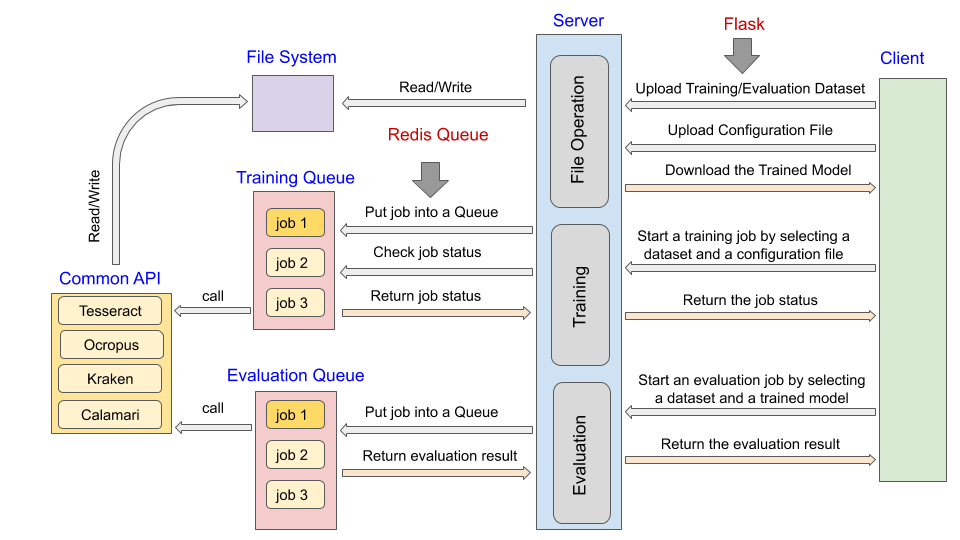
\includegraphics[width=0.8\linewidth]{Figures/Framework.png}
        \end{center}
        \caption{\small{Framework of the okralact system.}}
\label{fig:framework}
\end{figure*}

\section{Preliminary evaluation}

% CN: Before we conclude, I would expect another section with some
% minimal evaluation/results discussion, e.g. was it (not?)
% possible to a) train models for all four engines and b) using the
% same data according to specs with okralact and c) how do these
% models compare to ones that are shipped with each engine? 

% kba: Rui?

\section*{Challenges and Future Work}

% * [X] Adapt diagram \url{https://docs.google.com/presentation/d/1jyV7pWGkIgtIrc9uJ5jbUwNthOk0JSUgT_tA2QudwkA/edit#slide=id.p}
% * [X] Describe HTTP API
%   * [X] Draft a `/evaluation` endpoint taking evaluation config, model, groundTruth and %returning measures like CER, WER ...

% Expanded Common API by engine developers cooperating

Though we strived to harmonize the engine APIs into a common API,
there still remain many engine-specific parameters. Therefore,
effective use of \textit{okralact} at this stage requires knowledge
of the individual engine's implementation, making the common API a
``leaky abstraction''. We hope to encourage engine developers and
intend to involve ourselves in discussions about unified
terminology, data types and exchange formats to improve engine
interoperability and therefore make \textit{okralact} more
accessible to non-expert users.

% Cleanly defined evaluation measures necessary (no more ISRI or character-counting CER)

Furthermore, there is a sore lack of easy to use tools with well
defined measures for the evaluation of OCR. Traditionally, the
character error rate (CER) and to a lesser extent word error rate
(WER) have been the ratios to measure accuracy. However, these
measures require perfect GT and results can be misleading for
breakdowns in preprocessing such as segmentation errors or
technical flaws in model preparation such as characters not part
of the encoding.
% kba: Can we cite some State of the Art evaluation papers here to
% show that this is being worked on?

% CN: Well, CER/WER is still most prominent in IAPR. Within READ/Transkribus apparently they also still use BoW/CER/WER: https://github.com/CITlabRostock/CITlabErrorRate. One could of course argue for the inclusion of ReadingOrder in the evaluation, for necessary normalizations of encodings, how to deal with (and which) stopwords, but I am not really aware of any concerted efforts in this direction. TBH, the whole claim that evaluation methods and metrics need updating is not entirely clear to me once I abandon the perspective that it is simply too cost- and time-intensive to produce large amounts of GT?

% More flexible choice of input data (multiple works, individual lines from individual pages etc.)

% Integration of training workflow and recognition workflows

Lastly, we strive for a better integration of training and
recognition workflows. As \textit{okralact} is part of the OCR-D
ecosphere, which has been developing components of a full-stack
OCR workflow, including image preprocessing, layout detection, font
detection, layout classification, recognition and language-model
post-processing, we intend to integrate \textit{okralact} into the
OCR-D specification and reference implementation. This will enable
users to pick and choose the best Free Software implementations for
the hole gamut of text recognition needs.

% kba: Plug our module projects by citing papers here.


%\section*{References}

% Please number citations consecutively within brackets \cite{b1}. The
% sentence punctuation follows the bracket \cite{b2}. Refer simply to the reference
% number, as in \cite{IEEEexample:bluebookbook} ---do not use ``Ref. \cite{b3}'' or ``reference \cite{b3}'' except at
% the beginning of a sentence: ``Reference \cite{b3} was the first $\ldots$''
%
% Number footnotes separately in superscripts. Place the actual footnote at
% the bottom of the column in which it was cited. Do not put footnotes in the
% abstract or reference list. Use letters for table footnotes.
%
% Unless there are six authors or more give all authors' names; do not use
% ``et al.''. Papers that have not been published, even if they have been
% submitted for publication, should be cited as ``unpublished'' \cite{b4}. Papers
% that have been accepted for publication should be cited as ``in press'' \cite{b5}.
% Capitalize only the first word in a paper title, except for proper nouns and
% element symbols.
%
% For papers published in translation journals, please give the English
% citation first, followed by the original foreign-language citation \cite{b6}.

\bibliographystyle{IEEEtran}
\bibliography{bibliography}

\end{document}
